\subsection{Tools for Automatic Static Analysis}
All tools were run on the function \texttt{send\_publish\_notifications(..)} and on the file \texttt{tools.py}.

\subsubsection{Pylint}
The Python quality checker \emph{Pylint} is a tool to help with coding standard as recommended by PEP 8, error detection and refactoring.
Pylint message categories:
\begin{itemize}
    \item (C) convention: programming standard violation
    \item (R) refactor: code smell
    \item (W) warning: python specific problem
    \item (E) error: likely bug
    \item (F) fatal: an error occurred preventing pylint from continuing the analysis
\end{itemize}
\begin{figure}[h]
    \centering
    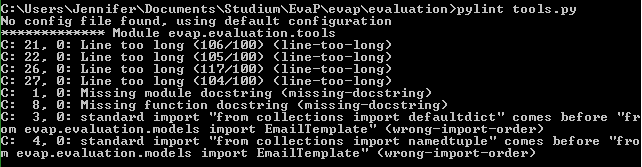
\includegraphics[width=\textwidth, keepaspectratio]{graphics/pylint_send_publish_notifications_1}
    \caption{Pylint messages for \texttt{send\_publish\_notifications(..)}}
    \label{fig:pylint}
\end{figure} 
As expected after our testing Pylint found mostly violated coding conventions in \texttt{send\_publish\_notifications(..)} (\ref{fig:pylint}).
The investigation of the file \texttt{tools.py} leads to a few warnings and refactoring hints that we will discuss with the developers on the next occasion.
%TODO Restliche Grafiken in den Anhang?


\subsubsection{Pychecker}
Even though you still find some outdated recommendations this tool's peak seems to be over. 
The last update was in 2013.
It is written for Python 2.x and has never been ported to Python 3.x.
Since the installation process requires Python 2.x while we work with Python 3.x in EvaP we will drop our investigation with this tool.

\subsubsection{pep8}
The Python style guide checker \emph{pep8} checks code against some of the style conventions in PEP 8.
It differentiates between errors and warnings.
\begin{figure}[h]
    \centering
    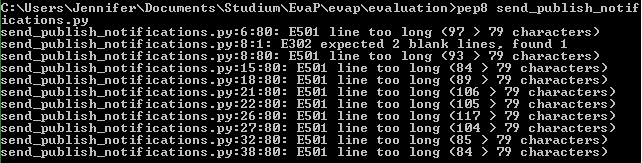
\includegraphics[width=\textwidth, keepaspectratio]{graphics/pep8_send_publish_notifications_1}
    \caption{pep8 messages for \texttt{send\_publish\_notifications(..)}}
    \label{fig:pep8}
\end{figure} 
pep8 throws a few more errors about lines being too long, because the line length was set to 100 instead of 80 characters in Pylint.

\subsubsection{Pyflakes}
Unlike Pylint and pep8 \emph{Pyflakes} does not check for violations of coding style but instead focuses on checking for errors.
The tool is less intuitively to use as there is no report if no errors are found. 
It did not report any errors for neither \texttt{send\_publish\_notifications(..)} nor \texttt{tools.py}

\subsubsection{Landscape}
As described above the service Landscape is currently deployed in the development process. 
The service advertises to find errors, possible problems and security issues.
Every time the master branch of the repository is updated Landscape runs several code quality tools including pylint on the whole codebase. 
It accumulates the findings, creates an easy access to them.
A rating based on the findings helps to get an overall idea about the current status.

\begin{figure}[h]
    \centering
    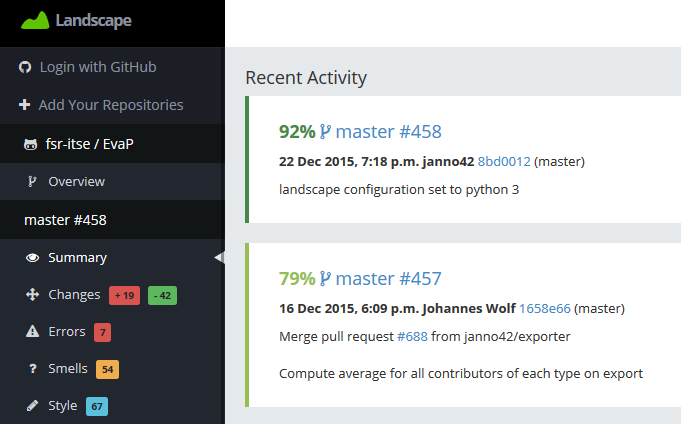
\includegraphics[width=0.7\textwidth, keepaspectratio]{graphics/landscape_python3}
    \caption{Landscape's rating of the code after changing the configuration from Python 2.x to Python 3.x}
    \label{fig:landscape_python3}
\end{figure} 

During our first investigation of the tool, we noticed that something was off about its configuration.
The last run was in %TODO
even though code was pushed to the master branch since then.
Additionally Landscape was still configured to run its checks against Python 2.x while EvaP already made the switch to Python 3.x.
Thankfully a fix of the configuration gave a significant boost to the rating (\autoref{fig:landscape_python3}).

\begin{figure}[h]
    \centering
    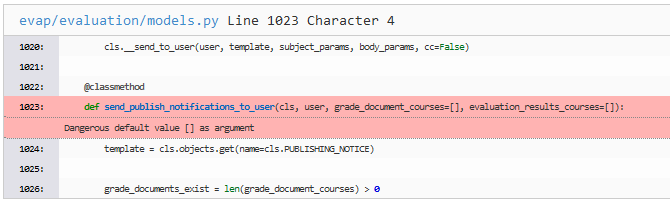
\includegraphics[width=\textwidth, keepaspectratio]{graphics/landscape_error}
    \caption{Landscape's display of an error found with static analysis}
    \label{fig:landscape_error}
\end{figure}

As we checked out the errors found section, we noticed that one of the found errors actually might have an impact on our test example function \texttt{send\_publish\_notifications}.
Landscape notified that the method \texttt{send\_publish\_notifications\_to\_user} has a dangerous default value as an argument.
(\autoref{fig:landscape_error})
In production, this method is called by our function, during testing we mocked it.

In the problematic code, a developer decided to make the function's arguments optional.
As both arguments are expected to be lists, he wanted the default argument to be empty lists.
The expected behavior was, that when the function is called without the respective arguments, the missing arguments would be set to empty lists.
Python however parses the definition of the function when initially parsing the file.
This is also when the default arguments are evaluated, therefore instead of creating new empty lists as default parameters on each execution of the function, those lists are only created once.

The found code problem is obviously a fault, but it does never become an error or failure in the current system, as the function neither adds values to passed lists, nor is it called more than once during one script execution.
But if future usages of the function --- within EvaP or another project --- would change that, the fault could potentially become an error and failure.

A possible fix for the fault is to set the default arguments to \texttt{None}, and to create empty lists inside the function's body, as can be seen in \texttt{send\_publish\_notifications}.

\subsubsection{PyCharm}
The static analyses that can be conducted with PyCharm far outreach the possibilities of the other tested tools.
Not only allows the IDE to search for possible faults in several types of source code (i.e. python, JavaScript, HTML, CSS, Django templates), but it also suggests automatic refactoring to solve these issues.

All found code issues are classified by their severity into the categories `Server problem`, `Typo`, `Info`, `Weak Warning`, `Warning` and `Error`.
One can both customize the type of issues and the severity of those that should be found by PyCharm.
This is an important feature as --- whilst providing good inspections for a series of possible faults --- PyCharm tends to be pessimistic inaccurate.
As PyCharm offers to find issues of around 400 types (a number that even can be increased with additional IDE plugins), the result list of the inspection is rather long and verbose when it is run with default settings.
Especially concerning the English language checks, PyCharm heavily tries to match all occurring words with spelling rules.
When it comes to variable names, this is often misleading and tends to produce loads of false positives. (\autoref{fig:pyCharmInspection-resultSummary})

\begin{figure}[h]
	\centering
	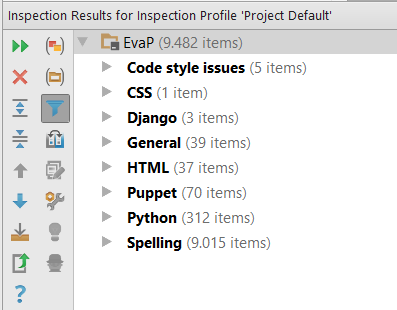
\includegraphics[width=0.4\textwidth]{graphics/pyCharmInspection-resultSummary}
	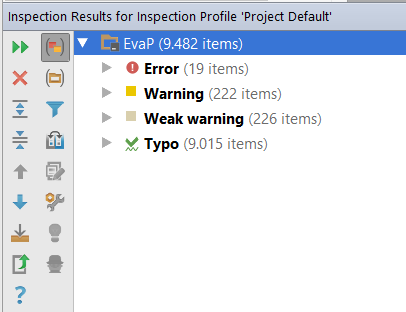
\includegraphics[width=0.4\textwidth]{graphics/pyCharmInspection-resultSummaryClassification}
	\caption{With the default configuration, PyCharm finds almost 9.5 thousand issues in the EvaP project. Most of them are false positives.}
	\label{fig:pyCharmInspection-resultSummary}
\end{figure}

Included in the list of issue types are both style guide or code convention violations and possible bugs due to actual faults.
For example, PyCharm checks for complete source code documentation, makes assumptions on the developer's intentions in contrast to possible typing errors and tries to apply data flow analysis to find uninitialized or unused variables.

With the help of the PyCharm code inspection, 15 faults could easily be fixed by either automatic refactoring or simple manual changes.
These fixes included false missing HTML tags and wrong tag nesting, dangerous python variable initialization and comparison as well as minor code convention violations.
About a hundred additional code smells can be fixed with small effort.

In addition to code inspections, PyCharm analyses the module dependencies and suggests to update them if the used version is outdated.
This feature is roughly equivalent to the data provided by the online service \textit{Gemnasium}, that monitors the project's GitHub repository.

\subsection{Experiences summarized}
Out of the tested tools three were particularly useful.

\begin{itemize}
    \item Pylint is pretty verbose, but very helpful if you are working on adjusting one file to the style guide.
    Its report is especially nice because it delivers statistics about the previous and the current run to compare the improvements due to the last code changes.
    \item PyCharm is especially useful for developers, because its inspection leads to the source code itself.
    Additionally PyCharm suggests fixes for its findings which enhances and accelerates the process quite a lot.
    \item Landscape's advantage is its setup as a service. It allows everyone to get an overview over the code quality without installing a tool on their machine. Furthermore, its automatic run after every code change on the master allows comparison between two states.
\end{itemize}

It is unfortunate that a tool as PyChecker that has not been updated for a while and does not work for Python 3.x is still listed and even highly recommended.  
While the tools pep8 and Pyflakes were not outstandingly useful for us they seem to serve their purpose.

The tools' usefulness regarding testing differs as well:
\begin{enumerate}
    \item PyCharm is the most useful, because it is simultaneously the IDE
    \item Landscape is helpful as it does not only locate possible erros, but suggest why a tester should be rethink the code or write a test 
    \item pylint and pep8 are great, because a uniform code style helps new developers and testers to easily find into the project. 
\end{enumerate}
